\documentclass{article}

\usepackage{scribe}

\setseriestitle{Probabilistic Machine Learning and Inference}
\setscribecode{4}
\setauthname{Gurpreet Singh}
\setinstrname{Piyush Rai}
\setauthemail{guggu@iitk.ac.in}
\settitle{Multi-parameter models and their Inference}

\begin{document}
\makeheader

\begin{ssection}[1]{Multi-parameter Models}

	In the previous scribes, we had looked at the inference of the mean and the variance / precision parameters of a Normal distribtuion, however we assumed only one of them to be unkown and inferred the other. That assumption made the inference a lot easier, as it was for only a single parameter. \br

	However, most machine learning tasks often have more than one parameter, and hence multi-parameter problems are important to understand. For this scribe, we will consider only models with two unknown parameters, with a single label / prediction, however the idea remains the same for any other multi-parameter model. Some examples of such models are shown in Figure \ref{fig:multi-models}

	\begin{figure}[h!]
		\centering
		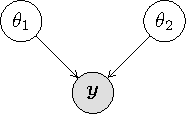
\includegraphics{includes/scribe04/multi-parameter-models-1.pdf}
		\hspace{2cm}
		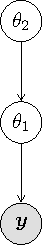
\includegraphics{includes/scribe04/multi-parameter-models-2.pdf}
		\hspace{2cm}
		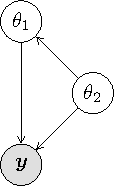
\includegraphics{includes/scribe04/multi-parameter-models-3.pdf}
		\caption{Plate Notations of multi-parameter models with two parameters}
		\label{fig:multi-models}
	\end{figure}

	Suppose we had to infer both the mean and the precision of a Gaussian Distribution jointly (two-parameter model), how would we do it? We will look at this example and its inference in the next section, and then mention some other more general solutions to inference.

\end{ssection}

\begin{ssection}[2]{A Simple Multi-parameter Model}

	Assume a one-dimensional Gaussian Distribution with unknown mean $\mu$ and precision $\lambda$. We have $n$ i.i.d. observations $X = \set{x^1, x^2 \dots x^n}$ sampled from this Gaussian \et{i.e}
	\begin{align*}
		\qforall i \in \brac{n},\; x^i \sim \ND{x^i \pipe \mu, \lambda^{-1}}
	\end{align*}

	We already know how to perform MLE estimation for such a problem. We simply need to equate the derivative of the MLE w.r.t. $\mu$ and $\lambda$ as we did for the coin-toss example (see Scribe 3). MLE estimation can, therefore, be a simple problem, even for multi-parameter models. \br

	We wish to infer the mean and the precision of this Gaussian using fully Bayesian Inference. Therefore, we need to compute the joint posterior of $\mu$ and $\lambda$. Let us first state the likelihood function $\para{\prob{X \pipe \mu, \lambda}}$ and the joint prior on $\mu$ and $\lambda$.
	\begin{align*}
		\mdef{Likelihood}	\prob{X \pipe \mu, \lambda}	&\eq	\prod_{i = 1}^n \sqrt{\frac{\lambda}{2 \pi}} \texp{- \frac{\lambda}{2} \para{x^i - \mu}^2} &
	\end{align*}

	In order to make the posterior tractable, we need to have a conjugate prior. In order to get an idea for that, let us represent the likelihood in a different manner
	\begin{equation}
		\prob{X \pipe \mu, \lambda}	&\qprop	\brac{\lambda^{\frac{1}{2}} \texp{- \frac{\lambda \mu^2}{2}}}^n \texp{\lambda \mu \sum_{i = 1}^n x^i - \frac{\lambda}{2} \sum_{i = 1}^n \para{x^i}^2}
		\label{eq:likelihood}
	\end{equation}

	Looking at Equation \ref{eq:likelihood}, we can say that the likelihood looks like a multiple of a gaussian and a gamma distribution. A similar form for the prior might prove to be a conjugate for the likelihood. In fact, we can precisely have such a distribution for the prior, known as the Normal-Gamma or the Gaussian-Gamma (NG) distribution.
	\begin{align*}
		\tfunc{NG}{\mu, \lambda \pipe \kappa_0, c, d}	&\qprop	\brac{\lambda^{\frac{1}{2}} \texp{-\frac{\lambda \mu^2}{2}}}^{\kappa_0} \texp{\lambda \mu c - \lambda d}
	\end{align*}

	\begin{remark}
		The multi-variate version of the Normal-Gamma distribution is known as the Normal-Wishart Distribution.
	\end{remark}

	\begin{remark}
		If we are doing inference for variance rather than precision, then we can use Normal-Inverse Gamma or for the multi-variate version, Normal-Inverse Wishart Distribution.
	\end{remark}

	It can be observed that the NG distribution has two terms, one which seems like a gaussian over $\mu$ and another which seems like a gamma distribution over $\lambda$. This can be better understood as when we marginalize over $\mu$ (\et{i.e.} integrate over $\mu$), we will get only the second term, that is the gamma over $\lambda$, since the gaussian over $\mu$ will integrate to one. Therefore, the gaussian term is just the conditional of $\mu$ over $\lambda$ and the gamma term is the marginal distribution of $\gamma$. \br

	More formally, we can write the NG distribution in the following representation
	\begin{equation}
		\tfunc{NG}{\mu, \lambda \pipe \mu_0, \kappa_0, \alpha_0, \beta_0, }	\eq	\prob{\mu \pipe \lambda} \prob{\lambda}	\eq	\ND{\mu \pipe \mu_0, \para{\kappa_0 \lambda}^{-1}} \tfunc{Gamma}{\lambda \pipe \alpha_0, \beta_0}
	\end{equation}

	where $\mu_0 = c / \kappa_0$, $\alpha_0 = 1 + \kappa_0 / 2$ and $\beta_0 = d - c^2 / 2\kappa$ \br

	Now, we can try to compute the posterior and show that the prior is indeed conjugate to the likelihood.

	\begin{ssubsection}{Computing the Posterior}

		\begin{align*}
			\prob{\mu, \lambda \pipe X}	&\eq	\frac{\prob{X \pipe \mu, \lambda} \prob{\mu, \lambda}}{\prob{X}} \\
										&\qprop	\prob{X \pipe \mu, \lambda} \prob{\mu, \lambda} \\
										&\eq	\prob{X \pipe \mu, \lambda}	\prob{\mu \pipe \lambda} \prob{\lambda}
		\end{align*}

		The complete derivation is much more involved and can be found in the paper by Murphy \cite{murphy-bayes}. However, we show the final form of the posterior as below. It is advised to try out the derivation as an exercise.
		\begin{align}
			\mdef{Posterior}	\prob{\mu, \lambda \pipe X}	&\eq	\tfunc{NG}{\mu_n, \kappa_n, \alpha_n, \beta_n} &
		\end{align}

		where
		\begin{align*}
			\mu_n			&\eq	\frac{\kappa_0 \mu_0 + n \overline{x}}{\kappa_0 + n} \\
			\kappa_n		&\eq	\kappa_0 + n \\
			\alpha_n		&\eq	\alpha_0 + \frac{n}{2} \\
			\beta_n			&\eq	\beta_0 + \frac{1}{2} \sum_{i = 1}^n \para{x^i - \overline{x}}^2 + \frac{\kappa_0 n \para{\overline{x} - \mu_0}^2}{2\para{\kappa_0 + n}} \\
			\overline{x}	&\eq	\frac{1}{n} \sum_{i = 1}^n x^i
		\end{align*}

		Hence, we have the posterior as a Normal-Gamma distribution, same as the prior.

	\end{ssubsection}

	\begin{ssubsection}{Completing the Inference}

		We can also compute some other quantities of interest, such as the predictive posterior and the margin likelihood. The marginal likelihood will have the following form \br
		\begin{align*}
			\mdef{Marginal Likelihood}	\prob{X}	&\eq	\frac{\Gamma(\alpha_n)}{\Gamma(\alpha_0)} \frac{\beta_0^\alpha_0}{\beta_n^\alpha_n} \para{\frac{\kappa_0}{\kappa_n}}^{\frac{1}{2}} (2 \pi)^{-\frac{n}{2}} &
		\end{align*}

		For this case, we have the predictive posterior as a student t-distribution, however we will not look at the derivation, which although can be found in the Murphy's paper \cite{murphy-bayes}
		\begin{align}
			\mdef{Predictive Posterior}	\prob{x^\ast \pipe X}	&\eq	\int_{\mu, \lambda} \prob{x^\ast \pipe \mu, \lambda} \prob{\mu, \lambda \pipe X}	\eq	t_{2 \alpha_n} \para{x^\ast \pipe \mu_n, \frac{\beta_n (\kappa_n + 1)}{\alpha_n \kappa_n}} &
		\end{align}

		We can also compute the marginal posteriors of $\mu$ and $\lambda$
		\begin{align*}
			\prob{\lambda \pipe X}	&\eq	\int_{\mu}	\prob{\mu, \lambda \pipe X}	\eq \tfunc{Gamma}{\lambda \pipe \alpha_n, \beta_n} \\
			\prob{\mu \pipe X}		&\eq	\int_{\lambda}	\prob{\mu, \lambda \pipe X}	\eq \func{t_{2 \alpha_n}}{\mu \pipe \mu_n, \beta_n / (\alpha_n \kappa_n)} \\
		\end{align*}

	\end{ssubsection}

\end{ssection}

\begin{ssection}{Handling the other cases}

	We analysed a very simple multi-parameter model, for which we could find a conjugate prior. However, for most of the machine learning problems, this is not the case \ie the posterior is generally intractable. Such a method would obviously fail in such a situation. \br

	To conquer these, we use sampling methods such as Monte Carlo Markov Chain (MCMC) and Variational Bayesian Inference (VI). These methods can approximate inference techniques using much weaker conditions than conjugacy, such as for MCMC methods, local conjugacy (more on this later) is required, whereas VI can be used even without that.

	Hence, the solution we discussed although powerful is infeasible for most of the problems. We will look at stronger methods as mentioned earlier later on in the series.

\end{ssection}

\vspace{10mm}
\begin{thebibliography}{10}

	\bibitem{murphy-bayes}
		Kevin P. Murphy
		\et{Conjugate Bayesian Analysis of the Gaussian Distribution, 2007}

\end{thebibliography}

\end{document}
